\documentclass[a4paper]{article}
\usepackage{graphicx}
\usepackage{amssymb}
\usepackage{fancyhdr}
\usepackage{hyperref}
\usepackage{lastpage}
\pagestyle{fancy}
\rhead{Andrea Vicari}
\lhead{Smart-IVC: Interactive Visualization of Cities}
\fancyfoot[C]{Page\ \thepage\ of\ \pageref{LastPage}}
\renewcommand{\headrulewidth}{0.4pt}
\renewcommand{\footrulewidth}{0.4pt}

\begin{document}

\begin{titlepage}

\newcommand{\HRule}{\rule{\linewidth}{0.5mm}} % Defines a new command for the horizontal lines, change thickness here

\center % Center everything on the page
 
%----------------------------------------------------------------------------------------
%	HEADING SECTIONS
%----------------------------------------------------------------------------------------
\textsc{\LARGE Universit\'a della Svizzera italiana}\\[1.5cm] % Name of your university/college
\textsc{\Large Faculty of Informatics}\\[0.5cm] % Major heading such as course name
\textsc{\large Bachelor Project Plan\\Spring Semester 2017}\\[0.5cm] % Minor heading such as course title

%----------------------------------------------------------------------------------------
%	TITLE SECTION
%----------------------------------------------------------------------------------------

\HRule \\[0.4cm]
{ \Huge \bfseries Smart-IVC}\\[0.4cm] % Title of your document
{ \huge Interactive Visualization of Cities}
\HRule \\[1.5cm]
 
%----------------------------------------------------------------------------------------
%	AUTHOR SECTION
%----------------------------------------------------------------------------------------

\begin{minipage}{0.4\textwidth}
\begin{flushleft} \large
\emph{Author:}\\
Andrea \textsc{Vicari} % Your name
vicara@usi.ch % Your name
\end{flushleft}
\end{minipage}
~
\begin{minipage}{0.4\textwidth}
\begin{flushright} \large
\emph{Advisor:} \\
Prof. Michele \textsc{Lanza} % Supervisor's Name
\emph{Assistant:} \\
Dr. Andrea \textsc{Mocci} % Supervisor's Name
\end{flushright}
\end{minipage}\\[4cm]

%----------------------------------------------------------------------------------------
%	DATE SECTION
%----------------------------------------------------------------------------------------

{\large \today}\\[3cm] % Date, change the \today to a set date if you want to be precise

%----------------------------------------------------------------------------------------
%	LOGO SECTION
%----------------------------------------------------------------------------------------


 
%----------------------------------------------------------------------------------------

\vfill % Fill the rest of the page with whitespace

\end{titlepage}

\section*{1. Motivation}
Web users have to aggregate different data from various sources whenever they are looking for some information on the Internet.

Think of the student who is looking for a rented room near his university: he uses a website to find an advertisement, then he looks for the address on another website to understand if the apartment is located near his university.


This spreading of information among various public entities and organizations, makes difficult to leverage them to support urban design and planning

\section*{2. Goal}
The goal of this Bachelor Project is to solve the issue presented above, creating a web application that uses information from various sources, combines them and provides a nice result to the user through a 3D map of the city that is also interactive.\\


\section*{3. Project Description}
For this bachelor project a web application is going to be created. It will both provide a 3D visualization of the urban environment of a city and integrate various sources of information about it, extracted for example from web resources.

The application will allow live interactions with entities (i.e. buildings) and the formulation of complex visual queries.


Clicking on a building on the map, the user will be able to both know more information about it (i.e. address, coordinates, number of floors etc.) and to formulate queries related to that entity, such as the distribution of important buildings like schools.
\section*{4. Plan}
\subsection*{Tasks and Milestones}
The tasks that will lead to the final result of this Bachelor Project are going to be the following:
\begin{itemize}
	\item {\bf Study Technologies} (1 week): choose the most suitable technologies for the project
	\item {\bf Build Back End} (2 weeks): retrieve data, model it, store the result in the database and create the APIs.
	\item {\bf Build Front-End GUI} (1 week): that consists in creating the basic skeleton of the website (i.e. menu and buttons) and it work with the APIs
\end{itemize}
Here I put the {\bf first milestone} (M1), therefore, by the end of March the Server and the basic GUI has to be ready.
\begin{itemize}
	\item {\bf Create 3D-Map} (4 weeks): create a 2.5D map and then add height to buildings and details to the map
	\item {\bf Create Interactions in 3D-Map} (3 weeks): make the entities on the map interactive clicking on them
\end{itemize}
Here I put the {\bf second milestone} (M2), therefore, by the first decade of May there must be a working 3D model of the city where is possible to execute queries on the entities
\begin{itemize}
	\item {\bf Test and Finish Work} (2 weeks): complete undone work, test the application and make the necessary fixes
	\item {\bf Write Thesis} (8 weeks): that includes writing the project report, the poster and the final plan
\end{itemize}
Here I present the graphical timeline of the tasks and milestones I described above:\\

\hspace*{-1cm}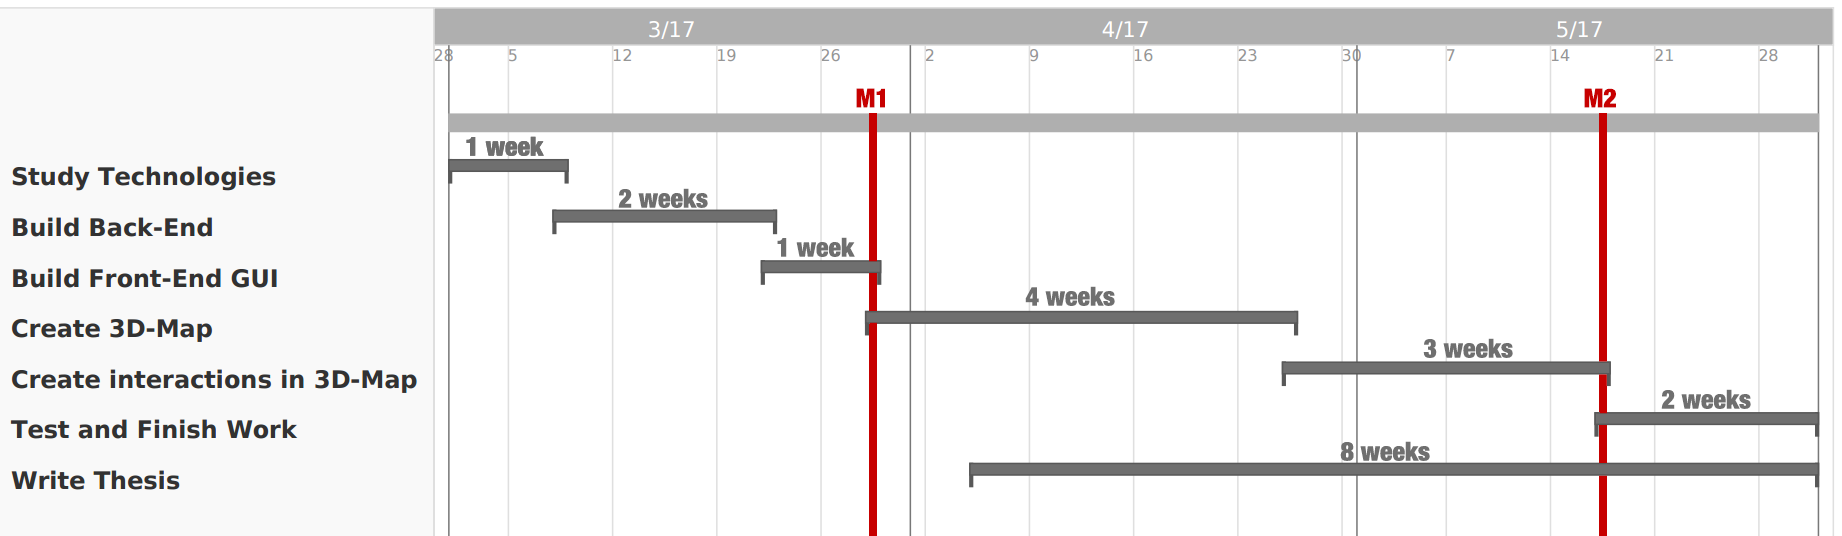
\includegraphics[scale=0.4]{Plan_timeline}
\\
\subsection*{Deliverables}
The deliverables that are going to be provided for this Bachelor Project are:
\begin{itemize}
	\item Project Report
	\item Poster
	\item Web Application
\end{itemize}

\end{document}
